
\clearpage
\setcounter{page}{1}
% \maketitlesupplementary
\appendix
\title{Cascade Prompt Learning for Vision-Language Model Adaptation\\Supplementary Material} 

\author{Ge Wu\inst{1}$^\dag$\orcidlink{0009-0008-3011-091X},
Xin Zhang\inst{1}$^\dag$\orcidlink{0009-0000-9078-9110},
Zheng Li\inst{1}\orcidlink{0000-0003-3309-1087},
Zhaowei Chen\inst{3}\orcidlink{0000-0002-9508-6999},
\\Jiajun Liang\inst{3}\orcidlink{0000-0001-5586-340X},
Jian Yang\inst{1}\orcidlink{0000-0003-4800-832X},
Xiang Li\inst{1,2}$^*$\orcidlink{0000-0002-4996-7365}
}

\footnotetext[1]{Equal contributions. Work is done when Ge Wu is an intern at Megvii Technology.}%
\footnotetext[2]{Corresponding author.}%

% TODO FINAL: Replace with an abbreviated list of authors.
\authorrunning{G. Wu et al.}
% First names are abbreviated in the running head.
% If there are more than two authors, 'et al.' is used.

% TODO FINAL: Replace with your institution list.
\institute{VCIP, CS, Nankai University 
\and NKIARI, Shenzhen Futian
\and Megvii Technology
\\ \email{gewu.nku@gmail.com, \{zhasion, zhengli97\}@mail.nankai.edu.cn, \\ \{csjyang, xiang.li.implus\}@nankai.edu.cn, \\ \{chenzhaowei, liangjiajun\}@megvii.com}
}


\titlerunning{Cascade Prompt Learning}

\maketitle

%\vspace{-12pt}

\section{Additional ablation studies}
%\vspace{-3pt}

\noindent{\textbf{Impact of training epoch for the first phase:}} 
% Fig.~\ref{fig:abalation-epochs} left depicts the influence of the number of training epochs in the first stage on CasPL performance using the DTD dataset. As the number of training epochs increases, the accuracy of the base class remains constant, while the accuracy of the novel class decreases after 20 epochs. 
Fig.~\ref{fig:abalation-epochs} (left) shows the impact of training epochs in the first stage on CasPL performance with the DTD dataset. The accuracy of the base class remains stable with increasing epochs, while the accuracy of the novel class decreases after 20 epochs.

\noindent{\textbf{Distillation temperature of learning boosting prompts:}}
% Table~\ref{table:ablation_temperature} shows the performance at different distillation temperatures. Generally, the best performance is achieved when the temperature parameter is 1. \zhangxin{ZX: I don't know how to analysize here.}
The temperature hyperparameter regulates the softness of the distributions. Therefore, in Fig.~\ref{fig:abalation-epochs} right, we examine the influence of employing different temperature hyperparameters to train boosting prompts in the first stage and then fine-tuning adapter prompts in the second stage, specifically on the DTD dataset. 
%The detailed configuration of PromptSRC + CasPL can be found in the appendix. 
According to the results, HM demonstrates the best performance when the temperature is set to 1. Hence, the temperature hyperparameter is default set to 1.


%%%%%%%%%%%%%%%%%%%%%%%%%%%%%%%%%%%%%%%%%%%%%%%%%%%%%%%%%%%%%%%%%%%%%%%%%%%%%%%%%%%%%%%
\begin{figure}[h]
	\centering
	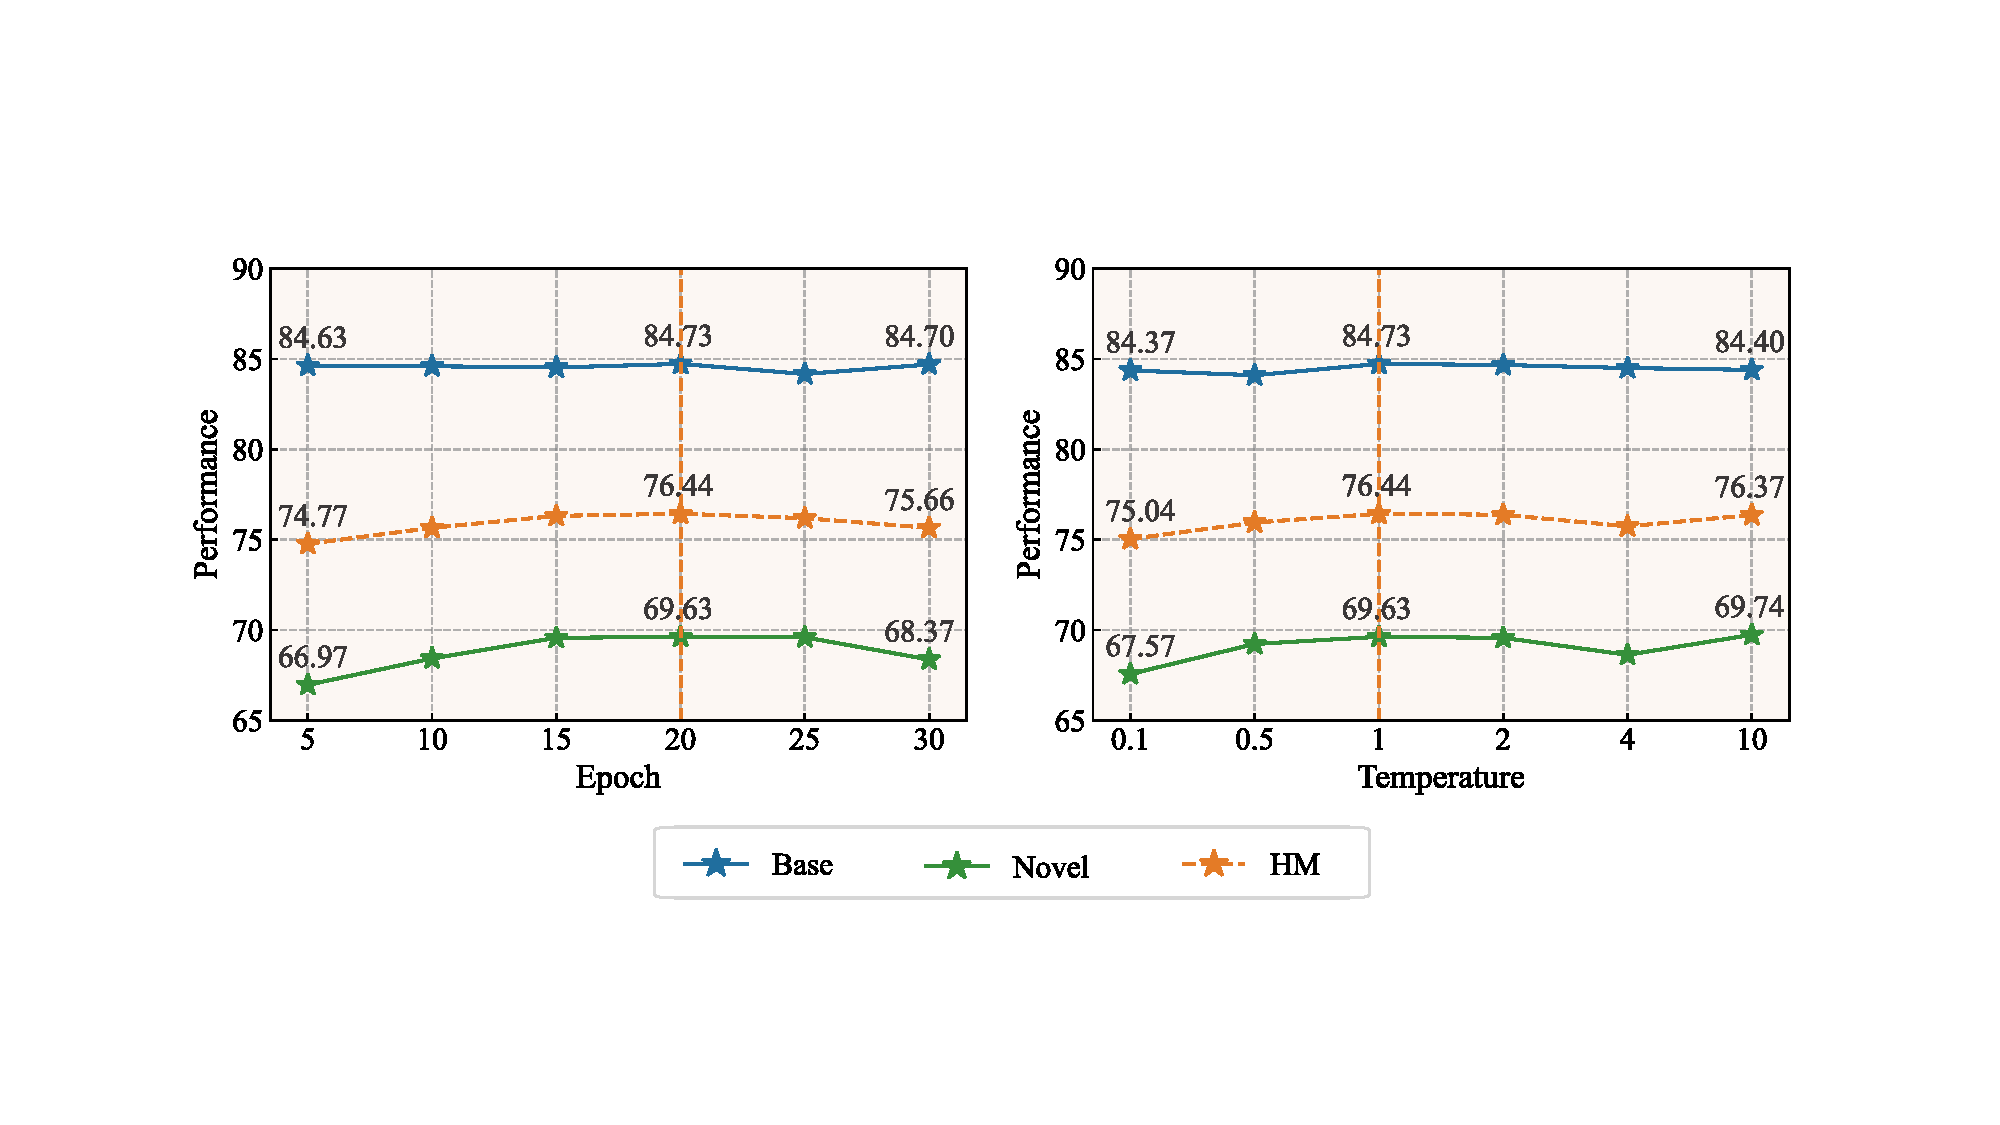
\includegraphics[width=0.7\linewidth]{fig/epoch_temperature.pdf}
    %\vspace{-10pt}
	\caption{Ablation study on the number of training epochs for the first phase (left) and the choice of temperature hyperparameter in Eq.~\eqref{eq_kd} (right), based on the DTD dataset.}
	\label{fig:abalation-epochs}
    %\vspace{-10pt}
\end{figure}
%%%%%%%%%%%%%%%%%%%%%%%%%%%%%%%%%%%%%%%%%%%%%%%%%%%%%%%%%%%%%%%%%%%%%%%%%%%%%%%%%%%%%%%


\noindent{\textbf{CLIP with boosting prompts for zero-shot inference:}}
Table~\ref{table:inference-domain} investigates the efficacy of integrating boosting prompts into CLIP for zero-shot inference. It demonstrates the accuracy improvement in domain generalization for CLIP (ViT-B/16)+ boosting prompt on both source and target datasets. However, solely using boosting prompts is less effective compared to our two-stage CasPL, as shown by the comparison with Table~\ref{table:base-to-novel}. This highlights the distinct roles played by the boosting prompts and the adapting prompts in our proposed framework.
% Table~\ref{table:inference-domain} explores the effectiveness of directly integrating boosting prompts into CLIP for zero-shot inference. Table \ref{table:inference-domain} showcases the accuracy of CLIP (ViT-B/16) + boosting prompt in domain generalization, with an increase in both source and target datasets. These findings suggest the success of boosting prompts in extracting domain-general knowledge through unsupervised knowledge distillation from a senior CLIP teacher. {However, based on the average results, employing only the boosting prompts is not as effective as our proposed two-stage CasPL, as indicated by the comparison with Table \ref{table:base-to-novel}. This observation underscores the distinct roles played by the boosting prompts and the adapting prompts in our proposed framework.}
%%%%%%%%%%%%%%%%%%%%%%%%%%%%%%%%%%%%%%%%%%%%%%%%%%%%%%%%%%%%%%%%%%%%%%%%%%%%%%%%%%%%%%%
%In Table \ref{table:inference}, CLIP (ViT-B/16) + boosting prompt achieves an average HM of 78.49$\%$ across 11 datasets, surpassing CLIP (ViT-B/16) with an HM of 71.70$\%$ by 6.79$\%$. Additionally, 

% \begin{table}[t]
%     \centering
%     \resizebox{0.8\linewidth}{!}
%     {
%         \begin{tabular}{clll}
%         \hline
%           Method     & Average  & ImageNet  &  Caltech101  \\
%         \hline
%         CLIP    &71.70   &70.22    &95.40    \\
%         \rowcolor{tablecolor}\textbf{+ boosting prompts}   &78.49  \improve{(+6.79)}    &73.62  \improve{(+3.40)}     & 96.20  \improve{(+0.80)}    \\
%         \hline
%           Method     & 	OxfordPets & Stanford Cars  & Flowers102  \\
%         \hline
%         CLIP    &94.12   &68.65    & 74.83   \\
%         \rowcolor{tablecolor}\textbf{+ boosting prompts}   &96.87 \improve{(+2.75)}    & 76.00  \improve{(+7.35)}    & 82.59  \improve{(+7.76)}    \\
%         \hline
%          Method      &  Food101 & 	FGVC Aircraft & SUN397  \\
%         \hline
%         CLIP    &90.66   & 31.09   & 72.23   \\
%         \rowcolor{tablecolor}\textbf{+ boosting prompts}   & 92.40   \improve{(+1.74)}  & 38.29 \improve{(+7.20)}     & 75.74 \improve{(+3.51)}     \\
%         \hline
%          Method      & DTD  &  EuroSAT & 	UCF101 \\
%         \hline
%         CLIP    &56.37   &60.03    &73.85    \\
%         \rowcolor{tablecolor}\textbf{+ boosting prompts}   &67.48  \improve{(+11.11)}    & 81.37 \improve{(+21.34)}     &81.54  \improve{(+7.69)}     \\
%         \hline
%         \end{tabular}
%     }
%     \vspace{10pt}
%     \caption{The HM of zero-shot inference utilizing CLIP (ViT-B/16) with the boosting prompts on base-to-novel generalization. Boosting prompts demonstrate the effectiveness of obtaining domain-general information from a senior CLIP teacher.}
%     \label{table:inference}
% \end{table}
%直接添加boosting prompts，对于domain的3个数据集也有涨幅，除了-A有掉点，其他都涨点
%直接添加boosting prompts，CLIP直接推理的novel好多都直接SOTA，比PromptSRC+CasPL的结果还高
%%%%%%%%%%%%%%%%%%%%%%%%%%%%%%%%%%%%%%%%%%%%%%%%%%%%%%%%%%%%%%%%%%%%%%%%%%%%%%%%%%%%%%%


\begin{table}[t]
    \centering
    \setlength{\tabcolsep}{10pt}
    \caption{The accuracy of zero-shot inference on domain generalization by CLIP (ViT-B/16) with adding boosting prompts. Boosting prompts can assist CLIP in enhancing domain generalization performance.}
    %\vspace{-5pt}
    \resizebox{0.9\linewidth}{!}
    {
        \begin{tabular}{cllll}
        % \hline\noalign{\smallskip}
        \hline
        \multirow{3}{*}{Method} & Source & \multicolumn{3}{c}{Target} \\
        \cmidrule(lr){2-2} \cmidrule(lr){3-5}
        & ImageNet & ImageNet-V2 & ImageNet-S  & ImageNet-R   \\
        \hline\noalign{\smallskip}
        CLIP & 66.73 & 60.83 & 46.15  & 73.96   \\
        \rowcolor{tablecolor}\textbf{+ boosting} & 70.40 \improve{(+3.67)}   &63.30 \improve{(+2.47)}   &47.70 \improve{(+1.55)}    &75.30 \improve{(+1.34)}     \\
        \hline
        \end{tabular}
    }
    \label{table:inference-domain}
    %\vspace{5pt}
\end{table}

\noindent{\textbf{Unsupervised training of boosting prompts using partial data:}}
This section investigates the impact of training boosting prompts with varying quantities of data on the outcomes of CasPL. Table~\ref{table:boost-few-shot} presents the DTD dataset's corresponding  HM values for different quantities. It is observed that, with an increase in the number of instances per category, the performance metric exhibits an overall upward trend, and PromptSRC +CasPL outperforms best through training on the entire dataset. Notably, when the instances per class are four or more, the HM of PromptSRC +CasPL ($\ge$72.31$\%$) exceeds that of PromptSRC HM (71.75$\%$), underscoring the effectiveness of boosting prompts.


%%%%%%%%%%%%%%%%%%%%%%%%%%%%%%%%%%%%%%%%%%%%%%%%%%%%%%%%%%%%%%%%%%%%%%%%%%%%%%%%%%%%%%%
% \begin{figure}[t]
% 	\centering
% 	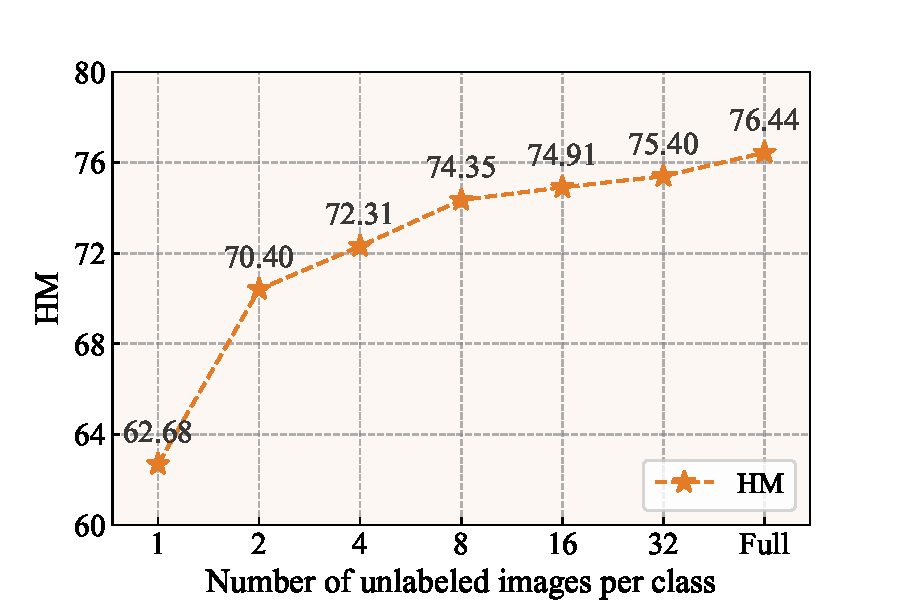
\includegraphics[width=0.45\linewidth]{fig/boost-few-shot.pdf}
%         \vspace{-5pt}
% 	\caption{\zhangxin{Ablation study on the HM results of boosting prompts trained with varying amounts of unlabeled images per class from the DTD dataset. (``Full'' indicates the utilization of the entire unlabeled dataset.) Utilizing more unlabeled data enables the boosting prompt to acquire more domain-general knowledge.}}
% 	\label{fig:boost-few-shot}
% \end{figure}
%%%%%%%%%%%%%%%%%%%%%%%%%%%%%%%%%%%%%%%%%%%%%%%%%%%%%%%%%%%%%%%%%%%%%%%%%%%%%%%%%%%%%%%

\begin{table}[t]
    \centering
    \setlength{\tabcolsep}{10pt}
    \caption{\zhangxin{Ablation study on the HM results of boosting prompts trained with varying amounts of unlabeled images per class from the DTD dataset. (``Full'' indicates the utilization of the entire unlabeled dataset.) Utilizing more unlabeled data enables the boosting prompt to acquire more domain-general knowledge.}}
    %\vspace{-5pt}
    \resizebox{0.85\linewidth}{!}
    {
        \begin{tabular}{c|lllllll}
            \hline
            Number & 1     & 2     & 4     & 8     & 16    & 32    & Full                      \\
            \hline
            HM     & 62.68 & 70.40 & 72.31 & 74.35 & 74.91 & 75.40 & \multicolumn{1}{r}{76.44} \\
            \hline
        \end{tabular}
    }
    \label{table:boost-few-shot}
    %\vspace{-5pt}
\end{table}

\section{Additional implementation details}
%\vspace{-3pt}
\subsection{Boosting prompt phase}
\noindent{\textbf{General training details:}}
For the first phase of CasPL, we train the boosting prompts with a layer depth of 12, prompt length of 8, and a learning rate of 0.0025 using the SGD optimizer for 20 epochs. All learnable prompts are initialized with a normal distribution. \zhangxin{To streamline the training of the boosting prompts on ImageNet, we utilize 8 NVIDIA 3090 GPUs, while all other experiments are conducted on a single NVIDIA 3090.}

\noindent{\textbf{Text templates for senior teacher CLIP}}
Drawing from previous findings~\cite{khattak2023self}, we utilize diverse prompt templates tailored to different datasets, aiming to augment the senior CLIP's text representation ability and enhance the boosting prompts' distillation effect. Table~\ref{table:templates} presents the templates for each dataset.
% According to prior research~\cite{khattak2023self}, we employ different prompt templates for various datasets to enhance the senior CLIP's text representation capability and improve the boosting prompts' distillation effect. Specifically, the corresponding template for each dataset is shown in Table~\ref{table:templates}.


\begin{table}[t]
    \centering
    \setlength{\tabcolsep}{15pt}    
    \caption{Text template utilized by senior CLIP teacher for different datasets.}
    %\vspace{-5pt}
    \resizebox{0.7\linewidth}{!}
    {
        \begin{tabular}{cl}
        \hline\noalign{\smallskip}
        \makecell[c]{Dataset} & \makecell[c]{Text template}\\
        \hline
        %ImageNet      & \textsf{`` a photo of a [class]. "}  \\
        %Caltech101    & \textsf{`` a photo of a [class]. "}      \\
        OxfordPets    & \textsf{`` a photo of a [class], a type of pet. "}      \\
        %Stanford Cars & \textsf{`` a photo of a [class]. "}      \\
        Flowers102    & \textsf{`` a photo of a [class], a type of flower. "}      \\
        Food101       & \textsf{`` a photo of [class], a type of food. "}     \\
        FGVC Aircraft & \textsf{`` a photo of a [class], a type of aircraft. "}      \\
        %SUN397        & \textsf{`` a photo of a [class]. "}     \\
        DTD           & \textsf{`` [class] texture. "}      \\
        EuroSAT       & \textsf{`` a centered satellite photo of [class]. "}     \\
        UCF101        & \textsf{`` a photo of a person doing [class]. "}      \\
        other datasets      & \textsf{`` a photo of a [class]. "}  \\
        %ImageNet-S    & \textsf{`` a photo of a [class]. "}  \\
        %ImageNet-V2   & \textsf{`` a photo of a [class]. "}  \\
        % ImageNet-A    & \textsf{`` a photo of a [class]. "}  \\
        %ImageNet-R    & \textsf{`` a photo of a [class]. "}  \\
        \hline
        \end{tabular}
    }
    % \vspace{-20pt}
    \label{table:templates}
\end{table}


\begin{figure*}[t]
	\centering
	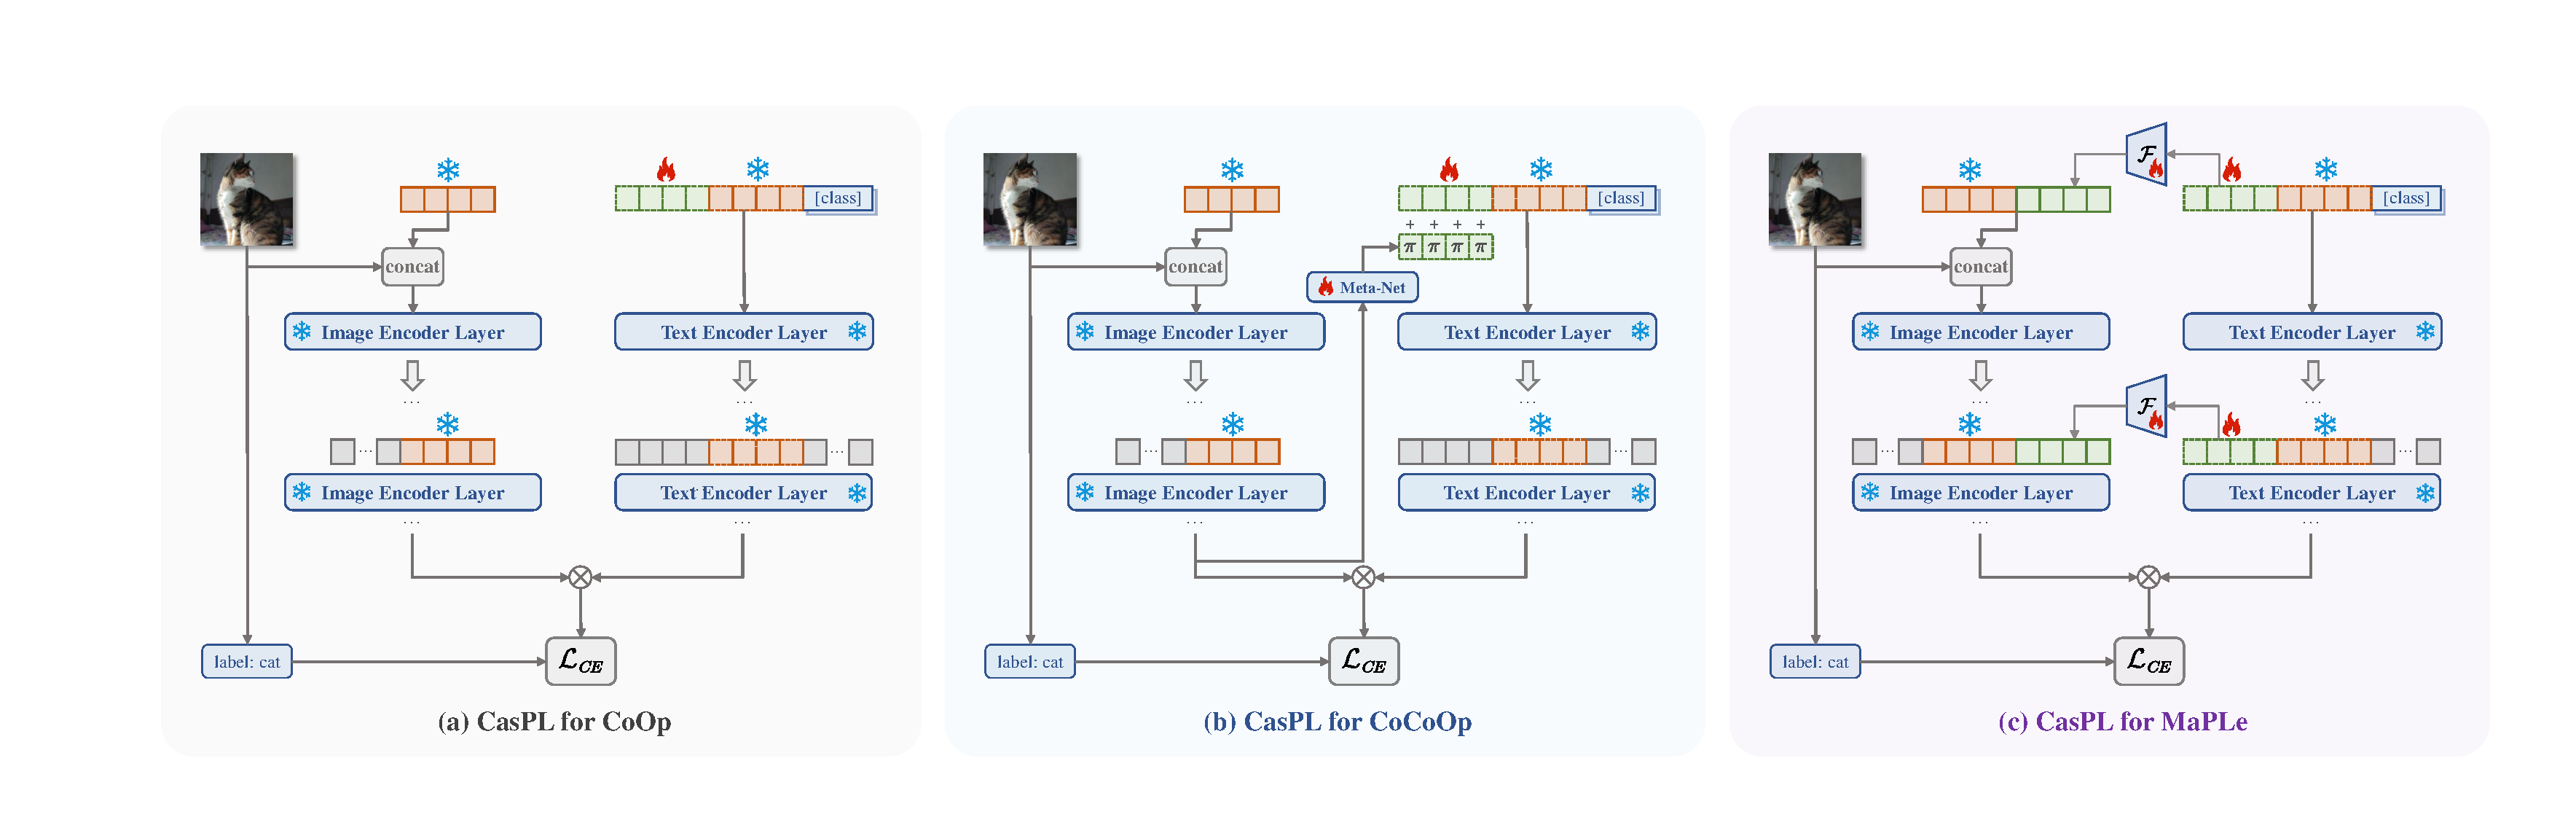
\includegraphics[width=1\linewidth]{fig/other_detail_eccv.pdf}
        %\vspace{-16pt}
	\caption{The detail of CasPL for previous methods. \indexbf{(a)} CoOp~\cite{zhou2022learning} employs multiple layers of text-image boosting prompts and a single layer of text adapting prompts. \indexbf{(b)} CoCoOp~\cite{zhou2022conditional} utilizes multiple layers of text-image boosting prompts and a single layer of modal blending adapting prompts. \indexbf{(c)} MaPLe~\cite{khattak2023maple} uses multiple layers of text-image boosting prompts and multiple layers of multi-modal adapting prompts.}
	\label{fig:methods-detail}
        %\vspace{-8pt}
\end{figure*}

\subsection{Adapting prompt phase}
\noindent{\textbf{Base-to-Novel generalization:}}
The training details of each of the previous methods on this task are shown in Table~\ref{table:training-setting}.
Various prior approaches based on prompt learning exhibit differences in the specifics of their implementation.
CoOp~\cite{zhou2022learning} employs single learnable text prompts (see Fig.~\ref{fig:methods-detail} (a)). CoCoOp~\cite{zhou2022conditional} combines image features with learnable text prompts to obtain multi-modal information (see Fig.~\ref{fig:methods-detail} (b)).  MaPLe~\cite{khattak2023maple} utilizes multi-layer learnable text prompts and image prompts generated from the text prompts (see Fig.~\ref{fig:methods-detail} (c)).  Specific details of PromptSRC are elaborated in Fig.~\ref{fig:framework}.

\noindent{\textbf{Domain generalization:}}
Following the previous method in this task~\cite{khattak2023maple}, we adjust the parameters for MaPLe, specifically setting its optimizer's learning rate to 0.0026 and establishing the training epoch at 2. 
%The remaining configurations align with those in Table~\ref{table:training-setting}.

\noindent{\textbf{Few-shot experiments:}}
% In alignment with the previously employed approach in this task~\cite{khattak2023self}, we designate the training epoch for PromptSRC as 50. The remaining configurations align with those in Table~\ref{table:training-setting}. The main text includes only the comparison curves, while more detailed numerical results are provided in Table~\ref{tab_appendix:few_shot_experiments}.
Following the methodology from previous work~\cite{khattak2023self}, we set the training epoch for PromptSRC at 50, keeping the other configurations consistent with those outlined in Table~\ref{table:training-setting}. The main text features comparison curves, while additional numerical results are available in Table~\ref{tab_appendix:few_shot_experiments}.


\noindent{\textbf{Compare with un-/weakly-supervised methods:}}
In this experiment, the CLIP zero-shot method utilizes simple templates as the text input, and the numerical results are derived from the official UPL~\cite{huang2022unsupervised} code.
To ensure a fair comparison, the three training strategies in ENCLIP~\cite{menghini2023enhancing} are implemented based on the PromptSRC pipeline~\cite{khattak2023self}. Few-pseudo labels (FPL) utilizes 16 pseudo labels per novel class and 16 labeled data per base class. Iterative Refinement of FPL (IFPL) utilizes the same training data as FPL but involves multiple iterations. The labels are recalculated in each iteration, and the prompt is reinitialized. Grow and Refine Iteratively Pseudolabels (GRIP) gradually increases the number of unlabeled datasets compared to IFPL (with a maximum limit of 16 per class in our implementation).


\begin{table}[t]
    \centering
    \setlength{\tabcolsep}{15pt}
    \caption{Training settings for base-to-novel generalization task.}
    %\vspace{-5pt}
    \resizebox{0.9\linewidth}{!}
    {
        \begin{tabular}{ccccc}
        \hline\noalign{\smallskip}
        ~& CoOp & CoCoOp & MaPLe & PromptSRC \\
        \hline
        Vision Prompt Length & - & - & 8 & 8 \\ 
        Text Prompt Length   & 8 & 8 & 8 & 8 \\ 
        Prompt Layer         & 1 & 1 & 12 & 12 \\ 
        Optimizer            & SGD & SGD & SGD & SGD \\ 
        Learning Rate        & 0.002 & 0.002 & 0.0035 & 0.0025 \\ 
        Epoch                & 50 & 10 & 5 & 20 \\
        \hline
        \end{tabular}
    }
    %\vspace{3pt}
    \label{table:training-setting}
\end{table}



% \begin{figure}[t]
% 	\centering
% 	\includegraphics[width=0.6\linewidth]{fig/ablation_small.pdf}
%         \vspace{-12pt}
% 	\caption{\zhangxin{Comparison between PromptSRC +CasPL (left) and PromptSRC +$\mathcal{L}_{KD}$ (right). PromptSRC +CasPL decouples the model's optimization objectives, utilizing different loss functions across different phases. In contrast, PromptSRC +$\mathcal{L}_{KD}$ uses multiple loss functions within a single phase, hindering model's efficient optimization.}}
% 	\label{fig:kd_describe}
% \end{figure}


% \section{Additional comparative trials}
% \noindent{\textbf{The details of ``+$\mathcal{L}_{KD}$'':}} 
% To provide a clearer illustration of ``+CasPL'' and ``+$\mathcal{L}_{KD}$'', we compare these two methods based on PromptSRC (see Fig.~\ref{fig:kd_describe}).
% Moreover, given the inconsistency of loss functions in different methods, a single-stage use of $\mathcal{L}_{KD}$ may yield varying effects. Therefore, we compare the four methods based on other previous approaches~\cite{zhou2022learning, khattak2023maple, zhou2022conditional, khattak2023self}, and the results are presented in Table~\ref{table:more_kd}. Generally, employing ``+CasPL'' results in better performance gains compared to ``+$\mathcal{L}_{KD}$''. 


% \begin{table}[t!]
%     \centering
%     \setlength{\tabcolsep}{10pt}
%     \caption{The performance of "+$\mathcal{L}_{KD}$" and "+CasPL" on various methods using the DTD dataset. CasPL outperforms $\mathcal{L}_{KD}$ across different methods, demonstrating the effectiveness of decoupling domain-general and task-specific knowledge.}
%     \vspace{-5pt}
%     \resizebox{.72\linewidth}{!}
%     {
%         \begin{tabular}{l|ccc}
%             \hline
%             Method                        & KD Teacher   & Phase  & HM \\
%             \hline
%             CoOp                           & \multirow{1}{*}{\makecell[c]{$\times$}} & single       & 54.24    \\
%             CoOp +$\mathcal{L}_{KD}$      & CLIP (ViT-L/14)   &    single    &64.23      \\
%             CoOp +CasPL                     & CLIP (ViT-L/14)     &  multi       & \textbf{65.47}   \\
%             \hline
%             CoCoOp                         & \multirow{1}{*}{\makecell[c]{$\times$}}  & single       & 64.85 \\
%             CoCoOp +$\mathcal{L}_{KD}$    & CLIP (ViT-L/14)    &     single    &65.37     \\
%             CoCoOp +CasPL                   & CLIP (ViT-L/14)    &  multi       & \textbf{70.35}   \\
%             \hline
%             MaPLe                          & \multirow{1}{*}{\makecell[c]{$\times$}}  & single       & 68.16 \\
%             MaPLe +$\mathcal{L}_{KD}$     & CLIP (ViT-L/14)    &     single     &71.03     \\
%             MaPLe +CasPL                    & CLIP (ViT-L/14)    &  multi       & \textbf{73.90}   \\
%             \hline
%             PromptSRC                      & \multirow{1}{*}{\makecell[c]{$\times$}}  & single       & 71.75 \\
%             PromptSRC +$\mathcal{L}_{KD}$ &  CLIP (ViT-L/14)    &   single      &  72.60  \\
%             PromptSRC +CasPL                &  CLIP (ViT-L/14)   &  multi          & \textbf{76.44}  \\
%             \hline
%         \end{tabular}
%     }
%     \vspace{10pt}
%     \label{table:more_kd}
% \end{table}


%\noindent{\textbf{Analysis of performance degradation on domain-datasets:}}
% \zhangxin{
% We aim to analyze whether the decrease in accuracy caused by our CasPL on ImageNet-S and ImageNet-R, compared with the vanilla PromptSRC in the domain generalization task, indicates a severe deterioration in model generalization. In Fig.~\ref{fig:domain-analyse}, we present samples sampled from ImageNet-V2 and ImageNet-Sketch, and the predicted probabilities under the two methods. It is evident that our CasPL introduces a shift in generalization, yet it still predicts the true class with a high probability (top3). We conduct a statistical analysis on such cases, and the results reveal that more than 81\% of the samples with incorrect predictions by our CasPL method, compared with the vanilla PromptSRC, still have the prediction probability of the true label in the top 3 across all categories. We can also observe a significant improvement in our method's ability to predict the correct class probability on ImageNet-V2. These indicate that our method does not significantly damage the generalization of the model.}
%In the Domain Generalization task, compared with the vanilla PromptSRC, our CasPL significantly improves performance on ImageNet-V2, but the performance on the ImageNet-Sketch is not satisfactory. In Fig.~\ref{fig:domain-analyse}, we present samples sampled from ImageNet-V2 and ImageNet-Sketch, along with the predicted probabilities under the two methods. We observe a notable enhancement in our method's ability to predict the correct class probability on ImageNet-V2. For ImageNet-Sketch, some samples are not classified correctly (top1) compared with the vanilla MaPLe, yet they still predict the true class with a high probability (top3). 
%A statistical analysis of such cases reveals that more than 81\% of the samples with incorrect predictions by our CasPL method, compared with the vanilla PromptSRC, still have the prediction probability of the true label in the top 3 across all categories. 

%Simultaneously, upon careful analysis of the predicted classes and probabilities, we discover that the predictions of CasPL seem to be reasonable from some aspects under the case of the absence of color, especially when color becomes the key to identifying a certain category.
%we observe that the absence of color information on ImageNet-Sketch introduces challenges to image classification. 
%For instance, the image labeled as \textbf{\emph{macaw}} is classified as \textbf{\emph{african grey parrot}}, which is considered somehow intuitive in the context of a grayscale image. 


%The performance of CasPL (built on PromptSRC) compared to other methods in the few-shot setting. Results across various few-shot setups demonstrate CasPL's ability to enhance model performance.
\begin{table*}[t!]
    \small \centering
    \setlength{\tabcolsep}{15pt}
    \caption{The performance of CasPL (built on PromptSRC) compared to other methods in the few-shot setting. Results across various few-shot setups demonstrate CasPL's ability to enhance model performance.}
    %\vspace{-5pt}
    \scalebox{0.63}[0.63]{
        \begin{tabular}{ll|ccccc}
        \hline
        Dataset & 
        Method & 
        1 shot &
        2 shots & 
        4 shots & 
        8 shots &
        16 shots \\  
        \hline
        \multirow{5}{*}{ImageNet}      & Linear probe CLIP      &32.13	&44.88&	54.85	&62.23	&67.31\\ 
                                       & CoOp                   &66.33	&67.07	&68.73	&70.63&	71.87\\ 
                                       & CoCoOp                  & 69.43	&69.78	&70.39&	70.63&	70.83\\
                                       & MaPLe                  & 62.67	&65.10	&67.70&	70.30&	72.33\\
                                       & PromptSRC             & 68.13	&69.77	&71.07	&72.33	&73.17\\
                                       \rowcolor{tablecolor}
                                       & CasPL \textbf{(Ours) }     &68.73   &70.07   &71.43    &72.87   & 74.20    \\
        \hline
        \multirow{5}{*}{Caltech101}    & Linear probe CLIP      & 79.88	&89.01	&92.05	&93.41	&95.43\\
                                       & CoOp                    & 92.60	&93.07	&94.40	&94.37	&95.57\\
                                       & CoCoOp                  & 93.83	&94.82	&94.98	&95.04	&95.16\\
                                       & MaPLe                  & 92.57	&93.97	&94.43&	95.20&	96.00\\
                                       &  PromptSRC              &93.67	&94.53	&95.27	&95.67	&96.07\\
                                       \rowcolor{tablecolor}
                                       & CasPL \textbf{(Ours) }    &93.97 	&95.20 	&96.10 	&96.23 	&96.80   \\
                                       \hline
        \multirow{5}{*}{DTD}           & Linear probe CLIP       & 34.59	&40.76	&55.71	&63.46	&69.96\\
                                       & CoOp                   &50.23&	53.60	&58.70	&64.77	&69.87\\
                                       & CoCoOp                      & 48.54	&52.17	&55.04	&58.89	&63.04\\
                                       & MaPLe                  & 52.13	&55.50	&61.00&	66.50&	71.33\\
                                       &  PromptSRC                  & 56.23&59.97	&65.53	&69.87	&72.73\\
                                       \rowcolor{tablecolor}
                                        & CasPL \textbf{(Ours) }    &62.63  &63.67 &69.07 &71.00 	&75.13      \\
                                       \hline
        \multirow{5}{*}{EuroSAT}       & Linear probe CLIP       &49.23	&61.98	&77.09&	84.43	&87.21\\
                                       & CoOp                   &54.93	&65.17	&70.80	&78.07	&84.93\\
                                       & CoCoOp                  & 55.33	&46.74	&65.56&	68.21	&73.32\\
                                        & MaPLe                  & 71.80	&78.30	&84.50&	87.73&	92.33\\
                                       & PromptSRC              &73.13 &79.37	&86.30	&88.80	&92.43\\
                                       \rowcolor{tablecolor}
                                        & CasPL \textbf{(Ours) }   &83.40 &86.53 	&91.07 	&91.07 	&94.17     \\
        \hline
        \multirow{5}{*}{StanfordCars}  & Linear probe CLIP     & 35.66	&50.28	&63.38	&73.67	&80.44\\
                                   & CoOp                        &67.43	&70.50	&74.47	&79.30	&83.07\\
                                           & CoCoOp              & 67.22	&68.37	&69.39	&70.44&	71.57\\
                                         & MaPLe                  & 66.60	&71.60	&75.30&	79.47&	83.57\\
                                      &  PromptSRC               &69.40	&73.40	&77.13	&80.97	&83.83\\
                                      \rowcolor{tablecolor}
                                       & CasPL \textbf{(Ours) }    &72.80 	&77.23 	&80.03 	&83.30 	&86.70     \\
        \hline
        \multirow{5}{*}{Flowers102}    & Linear probe CLIP      & 69.74	&85.07	&92.02	&96.10	&97.37\\
                                       & CoOp                   & 77.53	&87.33	&92.17	&94.97	&97.07\\
                                       & CoCoOp                    &72.08	&75.79	&78.40	&84.30	&87.84\\
                                       & MaPLe                  & 83.30	&88.93	&92.67&	95.80&	97.00\\
                                       & PromptSRC            & 85.93	&91.17	&93.87	&96.27	&97.60\\
                                       \rowcolor{tablecolor}
                                        & CasPL \textbf{(Ours) }  &90.33 &94.17  &95.53  &97.20  &98.30     \\
                                       \hline
        \multirow{5}{*}{FGVCAircraft}  & Linear probe CLIP       & 19.61	&26.41	&32.33	&39.35&	45.36\\
                                       & CoOp                     & 21.37&	26.20	&30.83	&39.00	&43.40\\
                                       & CoCoOp                   & 12.68	&15.06	&24.79	&26.61	&31.21\\
                                       & MaPLe                  & 26.73	&30.90	& 34.87&	42.00&	48.40\\
                                       & PromptSRC           & 27.67	&31.70	&37.47&	43.27	&50.83\\
                                       \rowcolor{tablecolor}
                                         & CasPL \textbf{(Ours) }   &32.80 &35.20 	&41.03 	&48.03 	&55.37  \\
                                       \hline
        \multirow{5}{*}{SUN397}        & Linear probe CLIP          & 41.58	&53.70	&63.00	&69.08	&73.28\\
                                       & CoOp                     & 66.77	&66.53	&69.97	&71.53	&74.67\\
                                       & CoCoOp                   & 68.33	&69.03&	70.21	&70.84	&72.15\\
                                       & MaPLe                  & 64.77	&67.10	&70.67&	73.23&	75.53\\
                                      & PromptSRC                &69.67	&71.60	&74.00	&75.73	&77.23\\
                                      \rowcolor{tablecolor}
                                       & CasPL \textbf{(Ours) }   & 71.03 	&72.70 	&74.53 	&76.33 &77.70      \\
                                       \hline
        \multirow{5}{*}{OxfordPets}    & Linear probe CLIP        & 44.06	&58.37	&71.17	&78.36	&85.34\\
                                       & CoOp                      & 90.37	&89.80	&92.57	&91.27	&91.87\\
                                       & CoCoOp                       & 91.27	&92.64	&92.81	&93.45	&93.34\\
                                       & MaPLe                  & 89.10	&90.87	&91.90&	92.57& 92.83\\
                                       & PromptSRC                   & 92.00	&92.50	&93.43	&93.50	&93.67\\
                                       \rowcolor{tablecolor}
                                        & CasPL \textbf{(Ours) }    & 92.97 	&93.37 	&93.97 &93.93 &94.13     \\
                                       \hline
        \multirow{5}{*}{UCF101}        & Linear probe CLIP        & 53.66	&65.78	&73.28	&79.34&	82.11\\
                                       & CoOp                     & 71.23	&73.43	&77.10	&80.20	&82.23\\
                                       & CoCoOp                   & 70.30	&73.51	&74.82	&77.14&	78.14\\
                                       & MaPLe                  & 71.83	&74.60	& 78.47& 81.37&	85.03\\
                                       & PromptSRC                   & 74.80	&78.50	&81.57	&84.30	&86.47\\
                                       \rowcolor{tablecolor}
                                        & CasPL \textbf{(Ours) }     &79.53 	&82.03 	&84.77 	&86.70 	&88.47      \\
                                       \hline
        \multirow{5}{*}{Food101}       & Linear probe CLIP       & 43.96	&61.51	&73.19	&79.79	&82.90\\
                                       & CoOp                    & 84.33	&84.40	&84.47	&82.67	&84.20\\
                                       & CoCoOp                     & 85.65	&86.22	&86.88	&86.97	&87.25\\
                                       & MaPLe                  & 80.50 &81.47	&81.77&	83.60&	85.33\\
                                       & PromptSRC                & 84.87&	85.70	&86.17	&86.90	&87.5\\
                                       \rowcolor{tablecolor}
                                        & CasPL \textbf{(Ours) }   &86.80 &87.20 	&87.40 	&87.80 	&88.40      \\
                                        \hline
        \multirow{5}{*}{Average}       & Linear probe CLIP       & 45.83	&57.98	&68.01	&74.47&	78.79\\
                                       & CoOp                    & 67.56	&70.65	&74.02	&76.98	&79.89\\
                                       & CoCoOp                & 66.79&	67.65	&71.21&	72.96	&74.90\\
                                       & MaPLe                  & 69.27	&72.58	&75.37&	78.89&	81.79\\
                                       & PromptSRC               & 72.32	&75.29	&78.35	&80.69	&82.87\\
                                       \rowcolor{tablecolor} 
                                       & CasPL \textbf{(Ours) } &  75.91 & 77.94  & 80.45& 82.22 & 84.49   \\
        
        \hline
        \end{tabular}
        }
    \label{tab_appendix:few_shot_experiments}
%\vspace{-5mm}
\end{table*}
%这个地方使用的配置是：output_1024_t_s_s1_int_v8_t8_s2_int_v8_t8_student_shots16


%%%%%%%%%%%%%%%%%%%%%%%%%%%%%%%%%%%%%%%%%%%%%%%%%%%%%%%%%%%%%%%%%%%%%%%%%%%%%%%%%%%%%%%
% \begin{figure}[t]
% 	\centering
% 	\includegraphics[width=0.95\linewidth]{fig/domain-analyse_eccv.pdf}
%         \vspace{-4pt}
% 	\caption{Visual comparison of predicted probabilities using MaPLe and MaPLe +CasPL methods. These highlight the efficacy of the two-stage decoupled training for cross-domain solid generalization.}
% 	\label{fig:domain-analyse}
%         % \vspace{30pt}
% \end{figure}
%%%%%%%%%%%%%%%%%%%%%%%%%%%%%%%%%%%%%%%%%%%%%%%%%%%%%%%%%%%%%%%%%%%%%%%%%%%%%%%%%%%%%%%


% \bibliographystyle{splncs04}
% \bibliography{main}
\end{document}
